\section{Ingestion module for the EDR file}

This sections describes the ingestion module for inserting the information of the link execution status files, which carry the reception status of the pass for both \acrshort{pedc} and \acrshort{bedc}.

The associated ingestion processors are:

\begin{itemize} 

\item \textbf{s2boa.ingestions.ingestion\_edrs\_link\_status.ingestion\_edrs\_link\_status}
  
\end{itemize}

This module uses the following \acrshort{dim} signatures:

\begin{itemize} 

\item \textbf{LINK\_EXECUTION\_STATUS\_SSS}: information of the link execution status reported by \acrshort{edrs} team.
  
\end{itemize}

The table \ref{tb:description_explicit_reference_ingestion_edrs_link_status} shows the description of the explicit references inserted by the ingestion.

\begin{longtable}{|M{0.3\linewidth}|M{0.55\linewidth}|}
\hline \textbf{Reference} & \textbf{Description} \\ \hline
\textbf{EDRS SESSION\_ID} & Identifier of the link execution status reported by \acrshort{edrs} team \\ \hline
\caption{Table describing the explicit reference associated to the ingestion}
\label{tb:description_explicit_reference_ingestion_edrs_link_status}
\end{longtable}

The figure \ref{fg:structure_ingestion_edrs_link_status} shows a simplified diagram of the structure of events inserted (associated structure of values not included for simplicity).

\begin{figure}[H]
  \begin{center}
	\centering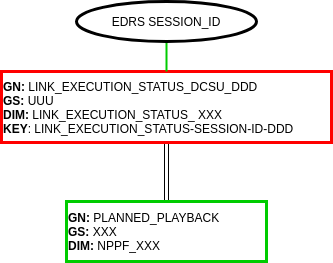
\includegraphics[scale=0.7]{../fig/structure_ingestion_edrs_link_status.png}
	\caption{Structure of events inserted by the ingestion module for the EDR file}
	\label{fg:structure_ingestion_edrs_link_status}
  \end{center}
\end{figure}

Where XXX is the corresponding satellite id, UUU is the \acrshort{edrs} unit DDD is the \acrshort{dcsu} id.

The table \ref{tb:description_events_ingestion_edrs_link_status} shows the description of the events inserted by the ingestion.

\begin{landscape}
\begin{longtable}{|M{0.15\linewidth}|M{0.05\linewidth}|M{0.10\linewidth}|M{0.10\linewidth}|M{0.15\linewidth}|M{0.15\linewidth}|M{0.15\linewidth}|}
\hline \textbf{Gauge name} & \textbf{Gauge system} & \textbf{DIM signature} & \textbf{Insertion mode} & \textbf{Description} & \textbf{Start} & \textbf{Stop} \\ \hline
\textbf{LINK\_EXECUTION\_STATUS\_DCSU\_DDD} & UUU & LINK\_EXECUTION\_STATUS\_SSS & EVENT\_KEYS (insert) [KEY: LINK\_EXECUTION\_STATUS-SESSION-ID-DDD] & Event for representing the information of the \textbf{link execution status reported by \acrshort{edrs}} team & UTC time associated to the validity start of the received file node & UTC time associated to the validity stop of the received file node  \\ \hline
\caption{Table describing the events associated to the ingestion}
\label{tb:description_events_ingestion_edrs_link_status}
\end{longtable}
\end{landscape}


